% !TeX program = xelatex
% !TeX encoding = UTF-8

\documentclass[xcolor=table,dvipsnames,svgnames,aspectratio=169]{beamer}

\usepackage{booktabs}
\usepackage{graphicx}
\usepackage{fontawesome5}
\usepackage{hyperref}
\usepackage{array}
\usepackage{tabularx}
\usepackage{colortbl}
\usepackage{makecell}
\usepackage{tikz}
\usetikzlibrary{matrix}

\graphicspath{{figures/}{story_map_assets/}}

\usetheme[min,blue]{sjtubeamer}
\titlegraphic{}
\setbeamertemplate{navigation symbols}{}

\title[Envoix · Story Map]%
  {\textbf{Envoix}: A Hybrid Adaptive Platform for Secure End-to-End File Transfer}
\subtitle{VE441 · Final Story Map and Initial Engine Architecture}
\author{Team NUUB}
\institute[SJTU GC]{Shanghai Jiao Tong University Global College}
\date{June 24, 2026}

\newcommand{\core}[1]{\textcolor{cprimary}{\textbf{#1}}}
\newcommand{\stagecell}[1]{\begin{minipage}[t]{\linewidth}\raggedright #1\end{minipage}}
\newcommand{\tightitems}{\setlength{\itemsep}{0.25em}\setlength{\parskip}{0em}}

\begin{document}

\maketitle

\begin{frame}[shrink=5]{Envoix --- Elevator Pitch}
  \begin{block}{}
    \centering\large\itshape
    Never waste time choosing how to send a file again ---\\
    Envoix pairs devices securely and automatically selects the fastest viable
    transfer path across LAN, direct Internet, peer-to-peer, relay, and
    encrypted store-and-forward conditions.
  \end{block}

  \vspace{1.0em}

  \begin{itemize}\tightitems
    \item \textbf{Zero decision cost} --- no manual choice between local transfer, cloud upload, relay, or command-line networking
    \item \textbf{Secure adaptive transfer} --- pairing, route selection, chunked resume, and BLAKE3 verification are engine-level behavior
    \item \textbf{Cross-platform core} --- shared Rust semantics first, then Android and Apple bindings
  \end{itemize}
\end{frame}

\begin{frame}{Team Members \quad{\small\normalfont\textbf{Team:} NUUB}}
\small
\renewcommand{\arraystretch}{1.14}
\begin{tabularx}{\textwidth}{@{}>{\bfseries}l l X@{}}
  \toprule
  Name & jAccount / uniqname & Task assignment \\
  \midrule
  Sun Qizhen & qz\_sun & Product architecture, adaptive routing engine, network path scoring. \\
  Zhang Jinbin & moranxuege & PM, mobile client direction, Android/iOS UX integration. \\
  Li Yuhao & 17521218310 & End-to-end encryption, QR/token handshake, secure session design. \\
  He Yumeng & y4954he & Relay server, deployment, network testing, fallback validation. \\
  \bottomrule
\end{tabularx}

\vspace{0.18em}
\begin{block}{Sub-team breakdown}
\footnotesize
Core engine: transport/session security and reliable transfer. Client integration:
CLI first, Android next. Relay/testing: fallback deployment and constrained-network validation.
\end{block}
\end{frame}

\begin{frame}{Core Value Proposition and UX Flow}
\small
\begin{columns}[T]
  \column{0.47\textwidth}
  \begin{block}{Core value proposition}
    For multi-device users who frequently move files across operating systems,
    Envoix automatically establishes a secure file-transfer session and selects
    the fastest available transfer path without accounts or manual tool choice.
  \end{block}

  \begin{alertblock}{Story-map scope}
    The map starts after Envoix is opened. It describes what the app does for
    the user --- features and capabilities --- rather than UI widgets.
  \end{alertblock}

  \column{0.49\textwidth}
  \large
  \begin{enumerate}\setlength{\itemsep}{0.75em}\setlength{\parskip}{0pt}
    \item Pair two devices --- no account.
    \item Detect available transfer paths.
    \item Select and establish the best path.
    \item Transfer file data securely.
    \item Recover from interruption; verify.
    \item Same behavior on desktop and mobile.
  \end{enumerate}
\end{columns}
\end{frame}

\section{Story Map}

\begin{frame}[fragile,shrink=8]{Story Map at a Glance}
\centering
\hyphenpenalty=10000\exhyphenpenalty=10000
\vspace{0.1em}
\begin{tikzpicture}[
  font=\small,
  M/.style={
    matrix of nodes,
    row sep=2pt, column sep=4pt,
    nodes={align=center, inner xsep=3pt, text height=2.0ex, text depth=0.7ex,
           minimum height=0.52cm, rounded corners=2.5pt, anchor=center},
    column 1/.style={nodes={text width=2.3cm, align=right, draw=none, fill=none, font=\small\bfseries}},
    column 2/.style={nodes={text width=3.45cm, draw=cprimary!45, fill=cprimary!8}},
    column 3/.style={nodes={text width=3.45cm, draw=csecondary!55, fill=csecondary!10}},
    column 4/.style={nodes={text width=3.45cm, draw=ctertiary!55, fill=ctertiary!10}},
  }
]
\matrix[M] (m) {
  & |[fill=cprimary,draw=cprimary,text=white,font=\small\bfseries]| Skeletal
  & |[fill=csecondary,draw=csecondary,text=white,font=\small\bfseries]| MVP
  & |[fill=ctertiary,draw=ctertiary,text=white,font=\small\bfseries]| Stretch \\
  Pair           & \core{One-scan pairing}   & Scan / link / code     & Multi-device invites \\
  Detect         & \core{LAN auto-discovery} & \core{Checks every route} & Network diagnostics \\
  Select         & \core{Fast path + relay}  & \core{Best path, live} & Works on locked nets \\
  Secure         & Encrypted connection      & \core{End-to-end crypto} & Traffic obfuscation \\
  Transfer       & \core{Reliable file send} & Android + desktop      & Folders, multi-file \\
  Resume         & \core{Resume + verify}    & Survives path switch   & Pause, parallel speed \\
  Cross-platform & Desktop apps              & Android parity         & iOS \& full releases \\
};
\end{tikzpicture}

\vspace{0.5em}
{\small\setlength{\fboxsep}{5pt}%
\fcolorbox{cprimary}{cprimary!8}{\core{Blue bold} = core technical barrier carrying the major project effort.}}
\end{frame}

\begin{frame}{Story Map --- Stage 1: Pair Devices}
\small
\renewcommand{\arraystretch}{1.42}
\begin{tabularx}{\textwidth}{@{}X X X@{}}
\toprule
\textbf{Skeletal Product} & \textbf{MVP} & \textbf{Stretch Goals} \\
\midrule
\stagecell{\core{Connect two devices by scanning one QR code --- no account, login, or contact list.\\
Invites expire; tampered, malformed, or weak invites are refused.}} &
\stagecell{Pair from a phone by scanning the code or tapping a link.\\
Type a short code when the camera is unavailable.\\
Clear ``paired and ready'' status.} &
\stagecell{Send to several people or devices from one invite.\\
Self-hosted invite delivery.\\
Stronger, independently audited pairing security.} \\
\bottomrule
\end{tabularx}
\end{frame}

\begin{frame}{Story Map --- Stage 2: Detect Paths}
\small
\renewcommand{\arraystretch}{1.42}
\begin{tabularx}{\textwidth}{@{}X X X@{}}
\toprule
\textbf{Skeletal Product} & \textbf{MVP} & \textbf{Stretch Goals} \\
\midrule
\stagecell{\core{Automatically find the other device on the local network.\\
Accept a typed or scanned address.\\
Give a clear error when no route is available.}} &
\stagecell{\core{Check every way to connect --- same network, direct Internet, peer-to-peer, relay, or encrypted offline drop-off --- and use whatever works.}} &
\stagecell{Diagnose restrictive or throttled networks.\\
Estimate connection quality (speed, delay, reliability) so users know what to expect.} \\
\bottomrule
\end{tabularx}
\end{frame}

\begin{frame}{Story Map --- Stage 3: Select Path}
\small
\renewcommand{\arraystretch}{1.42}
\begin{tabularx}{\textwidth}{@{}X X X@{}}
\toprule
\textbf{Skeletal Product} & \textbf{MVP} & \textbf{Stretch Goals} \\
\midrule
\stagecell{\core{Always try the fastest local connection first.\\
Fall back to a relay automatically.\\
No manual network setup.}} &
\stagecell{\core{Automatically pick the best available route --- local, direct, peer-to-peer, relay, or offline --- and show which one is in use.}} &
\stagecell{Keep working on locked-down networks.\\
Try options in parallel and use the fastest, most stable one.} \\
\bottomrule
\end{tabularx}
\end{frame}

\begin{frame}{Story Map --- Stage 4: Establish Secure Transport}
\small
\renewcommand{\arraystretch}{1.42}
\begin{tabularx}{\textwidth}{@{}X X X@{}}
\toprule
\textbf{Skeletal Product} & \textbf{MVP} & \textbf{Stretch Goals} \\
\midrule
\stagecell{Every transfer runs over an encrypted connection bound to the two paired devices.} &
\stagecell{\core{Files are end-to-end encrypted, so relays and offline servers can never see their contents.}} &
\stagecell{Disguise transfer traffic to keep working where ordinary transfers are blocked or throttled.} \\
\bottomrule
\end{tabularx}
\end{frame}

\begin{frame}{Story Map --- Stage 5: Transfer File Data}
\small
\renewcommand{\arraystretch}{1.42}
\begin{tabularx}{\textwidth}{@{}X X X@{}}
\toprule
\textbf{Skeletal Product} & \textbf{MVP} & \textbf{Stretch Goals} \\
\midrule
\stagecell{\core{Reliably send a file from one device to another with clear progress from start to finish.}} &
\stagecell{Send and receive on both Android and desktop with the same experience and live progress.} &
\stagecell{Send entire folders, many files at once, or run several transfers in parallel.} \\
\bottomrule
\end{tabularx}
\end{frame}

\begin{frame}{Story Map --- Stage 6: Resume and Verify}
\small
\renewcommand{\arraystretch}{1.36}
\begin{tabularx}{\textwidth}{@{}X X X@{}}
\toprule
\textbf{Skeletal Product} & \textbf{MVP} & \textbf{Stretch Goals} \\
\midrule
\stagecell{\core{Interrupted transfers pick up where they left off.\\
Every file is verified intact before it is saved --- no corrupted output.}} &
\stagecell{Files are checked continuously, and transfers keep going even when the connection switches networks mid-way.} &
\stagecell{Pause and resume whenever you want.\\
Faster transfers through parallel, self-tuning delivery.} \\
\bottomrule
\end{tabularx}
\end{frame}

\begin{frame}{Story Map --- Stage 7: Cross-Platform Delivery}
\small
\renewcommand{\arraystretch}{1.42}
\begin{tabularx}{\textwidth}{@{}X X X@{}}
\toprule
\textbf{Skeletal Product} & \textbf{MVP} & \textbf{Stretch Goals} \\
\midrule
\stagecell{Works as a desktop app on Windows, macOS, and Linux from one shared core.} &
\stagecell{An Android app with exactly the same pairing, transfer, resume, and verification behavior.} &
\stagecell{A native iOS/macOS app, plus packaged releases for every major platform.} \\
\bottomrule
\end{tabularx}

\vspace{0.45em}
\begin{block}{Core technical barriers}
\small
Adaptive path selection; secure pairing/session authentication; reliable stateful transfer; shared cross-platform core; relay/rendezvous/store-forward fallback.
\end{block}
\end{frame}

\section{Acceptance Criteria}

\begin{frame}[shrink=7]{Acceptance Criterion 1 --- Skeletal Product Feature}
\begin{block}{Authenticated stateful direct QUIC file transfer}
\small
\textbf{Given} two desktop Envoix clients using the same valid pairing token,
\textbf{when} the receiver listens on a reachable IPv4 or IPv6 address and the
sender requests one file transfer, \textbf{then} the session authenticates before
file metadata is sent, transfers the file in sequential chunks, persists
resumable receiver state in a \texttt{.part} file and JSON sidecar after
interruption, resumes from the recorded byte offset on restart, verifies the
final BLAKE3 hash, writes the final file only after verification, and returns a
successful transfer summary with the correct file name and byte count.
\end{block}

\begin{alertblock}{Done means}
\small
Expired, malformed, weak-token, or version-mismatched invites are rejected; no
unauthenticated metadata is sent; no partial or corrupted output is silently
promoted to the final file.
\end{alertblock}
\end{frame}

\begin{frame}[shrink=7]{Acceptance Criterion 2 --- MVP Feature}
\begin{block}{Automatic multi-path selection}
\small
\textbf{Given} sender and receiver clients with a valid pairing invite and at
least one viable network path, \textbf{when} automatic connection setup starts,
\textbf{then} Envoix probes supported strategies, attempts LAN/direct QUIC,
IPv6 direct QUIC, Internet P2P/hole punching, relay fallback, and encrypted
server store-and-forward according to priority and availability, emits the
selected strategy as a client event, keeps relay/server paths ciphertext-only,
and either completes the transfer or returns a clear no-path-available error
without creating a corrupted final file.
\end{block}

\begin{alertblock}{Done means}
\small
The user never chooses a network path manually. If the chosen path fails, the
engine tries the next viable path and resumes from compatible chunk state
instead of restarting from zero.
\end{alertblock}
\end{frame}

\section{Engine Architecture}

\begin{frame}{Engine Architecture --- Client Crate Dependencies}
\centering
\vspace{-0.2em}
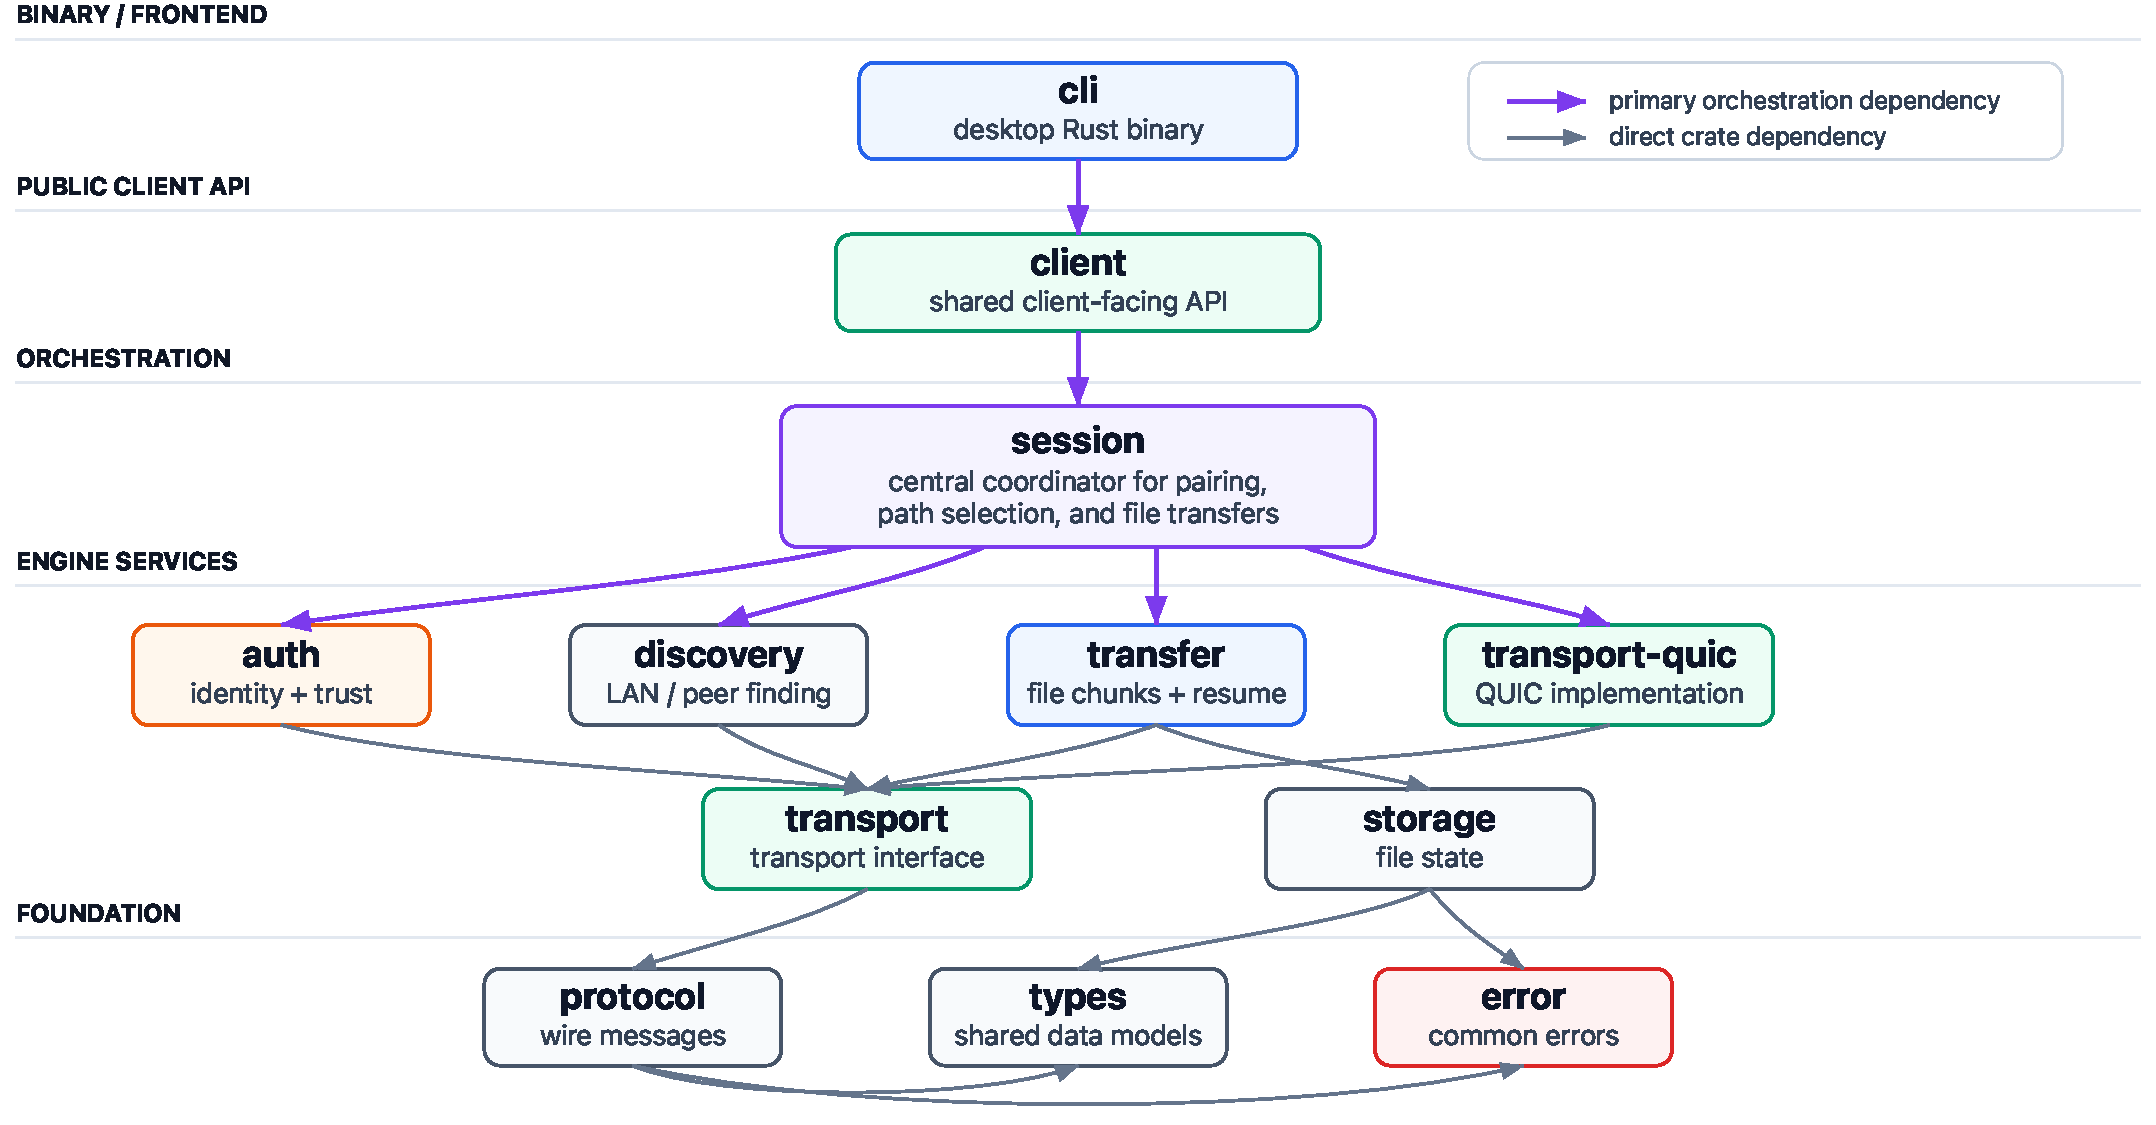
\includegraphics[width=\textwidth,height=0.86\textheight,keepaspectratio]{envoix_client_crate_dependencies.pdf}
\end{frame}

\begin{frame}{Engine Architecture --- Runtime Logic Flow}
\centering
\vspace{-0.2em}
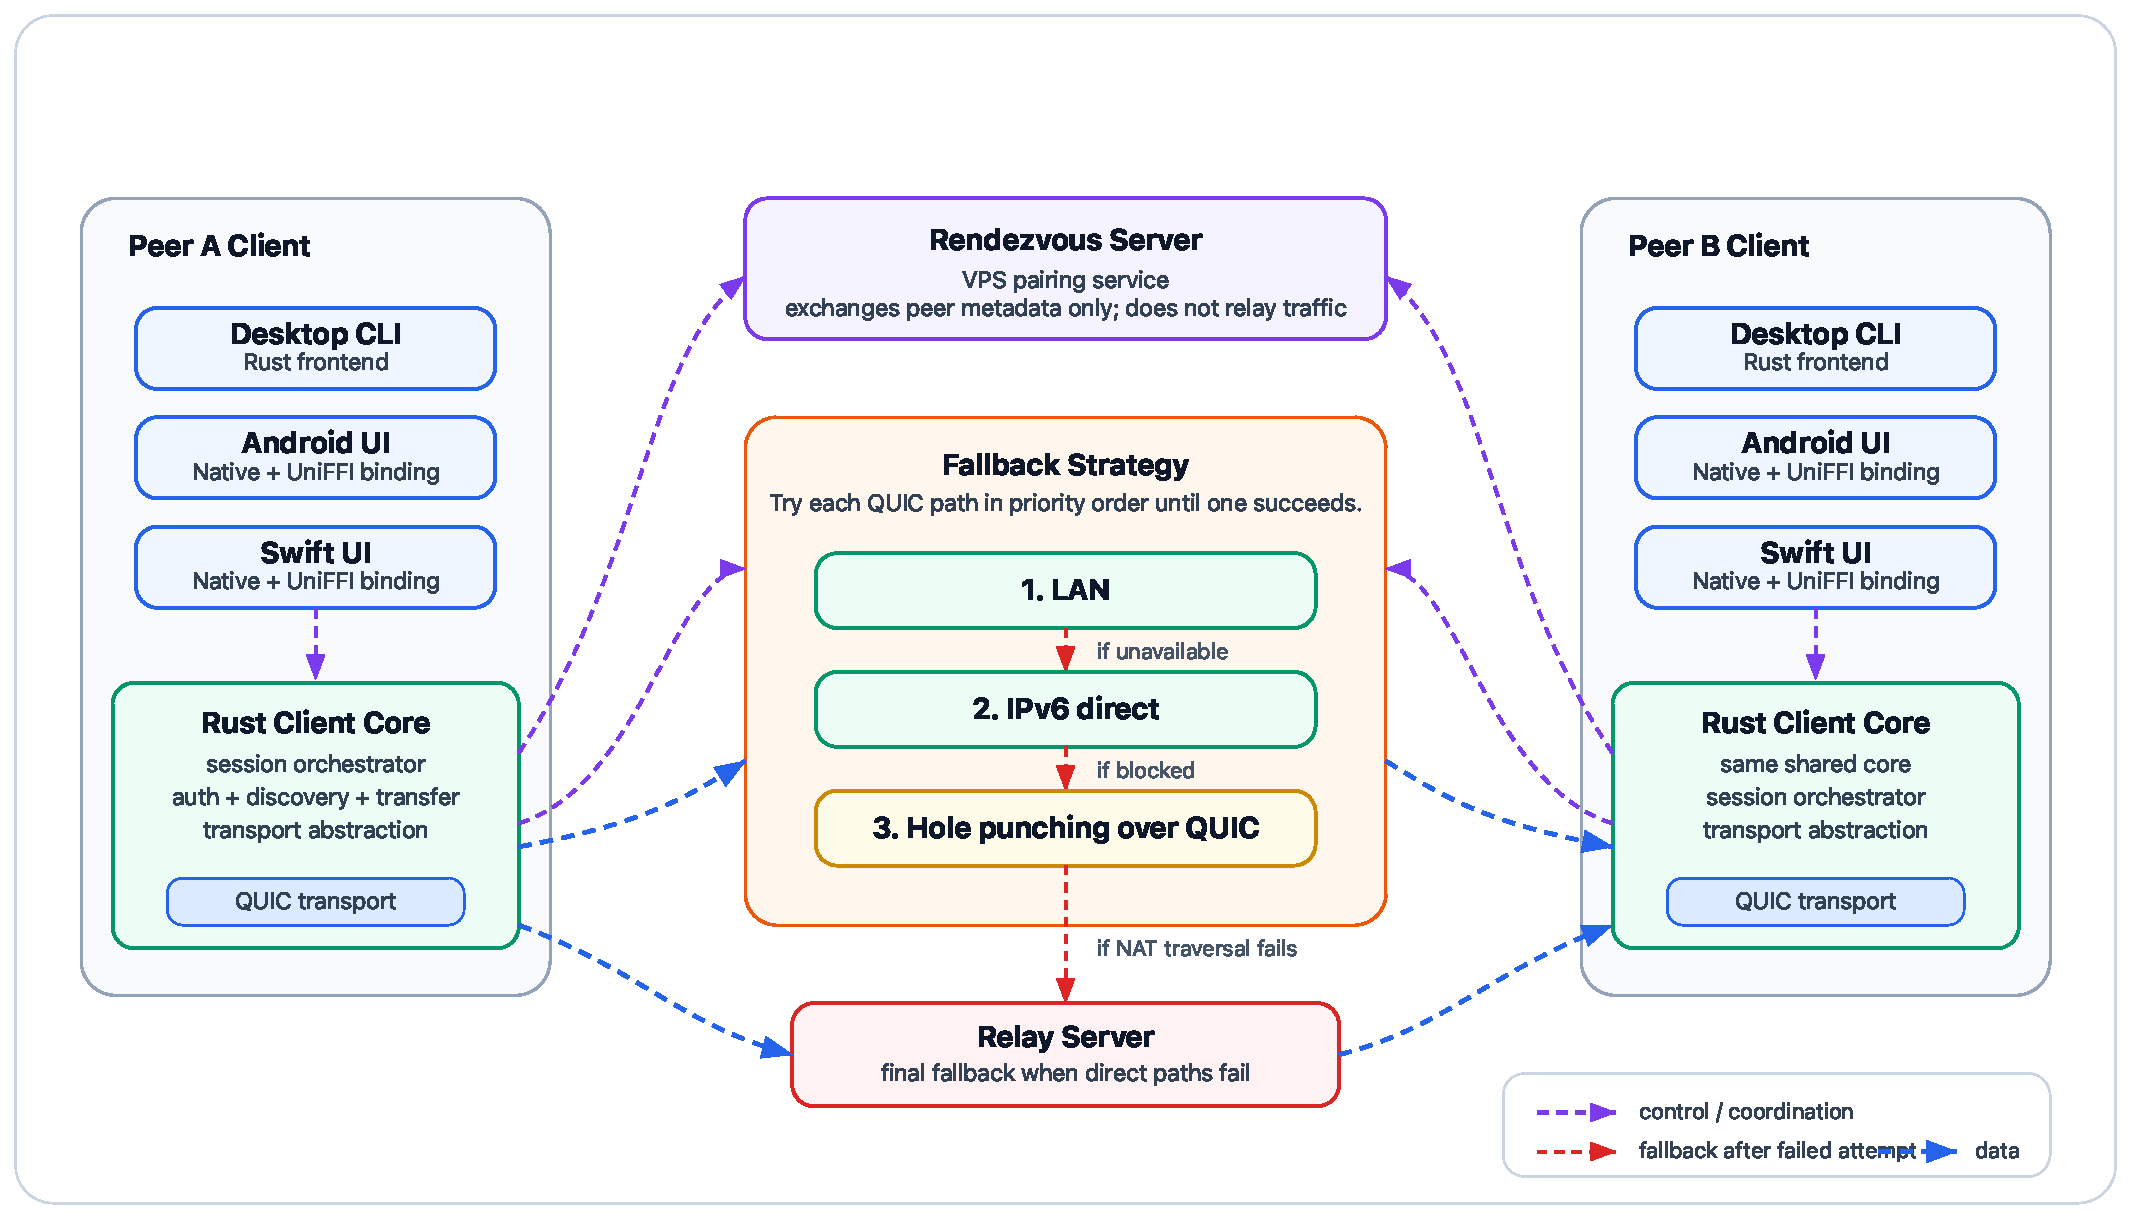
\includegraphics[width=\textwidth,height=0.86\textheight,keepaspectratio]{envoix_runtime_logic_flow_final.pdf}
\end{frame}

\begin{frame}[shrink=9]{Engine Components and Planned Tools}
\scriptsize
\renewcommand{\arraystretch}{1.12}
\begin{tabularx}{\textwidth}{@{}p{0.22\textwidth}X p{0.25\textwidth}@{}}
\toprule
\textbf{Component} & \textbf{Role in engine} & \textbf{Key tools / libraries} \\
\midrule
\texttt{envoix-client} & Public facade for send/receive requests, config validation, progress, selected-path, auth, and failure events. & Rust, typed client API \\
\texttt{envoix-session} & Orchestrates pairing, candidate selection, QUIC/relay setup, and transfer engine wiring. & Tokio async runtime \\
\texttt{envoix-auth} & SPAKE2 token pairing, confirmation MAC, channel binding, session-key derivation path. & SPAKE2, MAC, future audited PAKE review \\
\texttt{envoix-qr} & Invite serialization, expiry/version validation, token generation, QR rendering. & QR payload encoding/decoding \\
\texttt{envoix-transport} & Abstract connection traits so transfer logic is independent of QUIC, P2P, relay, or store-forward paths. & Trait-based Rust abstraction \\
\texttt{envoix-transport-quic} & Current concrete direct/LAN transport. & QUIC, TLS channel material \\
\texttt{envoix-transfer} & Protocol state machine, typed frames, chunk streaming, complete acknowledgements, events. & Length-prefixed JSON frame protocol \\
\texttt{envoix-storage} & \texttt{.part} output, resume sidecar, compatible-state validation, verified rename. & JSON sidecar, BLAKE3 hash \\
Relay / rendezvous / server & Candidate exchange, hole-punch metadata, relay fallback, encrypted store-and-forward. & Self-hostable relay, ciphertext-only forwarding \\
\bottomrule
\end{tabularx}
\end{frame}

\begin{frame}{Data and Control Flow Summary}
\footnotesize
\begin{columns}[T]
\column{0.48\textwidth}
\begin{block}{Control flow}
\begin{enumerate}\tightitems
  \item Client receives send/receive request.
  \item Session validates invite and token policy.
  \item Auth completes SPAKE2 and confirmation MAC.
  \item Strategy layer probes and ranks candidates.
  \item Session opens selected transport or fallback.
  \item Events report selected path, progress, failure reason, and completion.
\end{enumerate}
\end{block}

\column{0.48\textwidth}
\begin{block}{Data flow}
\begin{enumerate}\tightitems
  \item File metadata is sent only after authentication.
  \item Transfer engine emits typed protocol frames.
  \item Chunks move through QUIC, relay, or store-forward adapter.
  \item Receiver writes \texttt{.part} data and JSON resume sidecar.
  \item BLAKE3 verification gates final rename.
  \item Relay and server paths carry ciphertext only in the MVP design.
\end{enumerate}
\end{block}
\end{columns}
\end{frame}

\section{APIs and Controller}

\begin{frame}{APIs --- Front-End to Engine Boundary}
\small
Front ends call the \texttt{EnvoixClient} facade --- not the protocol, transport, or storage crates. Inputs are typed request models (\texttt{SendRequest}, \texttt{ReceiveRequest}, \dots).

\vspace{0.8em}
\renewcommand{\arraystretch}{1.35}
\begin{tabularx}{\textwidth}{@{}>{\raggedright\arraybackslash}p{0.46\textwidth}X@{}}
\toprule
\textbf{Public API} & \textbf{Role} \\
\midrule
\texttt{EnvoixClient::send} / \texttt{receive} & Automatic: discover over mDNS, select a path, authenticate, and transfer one file. \\
\texttt{send\_file} / \texttt{receive\_file\_with\_bound\_addr} & Manual: explicit socket address; bind, authenticate, transfer one file. \\
\texttt{ClientConfig::from\_runtime\_sources} & Load and validate configuration (chunk size, TOML, env) and pairing. \\
\texttt{ClientEventSink} / \texttt{EventSink} & Connection events (discovery, auth) and transfer events (progress, completion, failure). \\
\bottomrule
\end{tabularx}
\end{frame}

\begin{frame}{APIs --- Rendezvous Server (Signaling)}
\footnotesize
The rendezvous server only helps NAT-bound peers find each other. It exchanges connection candidates --- \textbf{never} file data --- and peers still run SPAKE2 first.

\vspace{0.5em}
\renewcommand{\arraystretch}{1.25}
\begin{tabularx}{\textwidth}{@{}>{\ttfamily\raggedright\arraybackslash}p{0.50\textwidth}X@{}}
\toprule
\normalfont\textbf{Endpoint} & \textbf{Purpose} \\
\midrule
POST /api/v1/sessions & Receiver registers a short-lived session. \\
POST /sessions/\{id\}/join & Sender joins with its capability token. \\
POST /sessions/\{id\}/candidates & Either peer publishes a typed QUIC candidate. \\
GET /sessions/\{id\}/candidates?since=N & Polls incremental candidates from the other peer. \\
DELETE /sessions/\{id\} & Receiver closes the session. \\
GET /api/v1/health & Unauthenticated liveness status. \\
GET /api/v1/stats & Authenticated operator statistics (when enabled). \\
\bottomrule
\end{tabularx}

\vspace{0.4em}
{\footnotesize Implemented in the server prototype; not yet wired into the integrated client.}
\end{frame}

\begin{frame}{\mbox{}}
\centering
\vfill
{\Huge\textcolor{cprimary}{\textbf{Thank You}}}\par
\vspace{1.0em}
{\large Team NUUB \quad\textbar\quad Envoix}\par
\vspace{0.4em}
{\normalsize Questions \& Discussion}
\vfill
\end{frame}

\end{document}
